\documentclass[11pt,english]{article}

% Set page margins correctly
\usepackage{geometry}
\usepackage{url}
\geometry{letterpaper,top=1.0in,left=1.0in,bottom=1.0in,top=1.0in,headsep=6pt,footskip=18pt}

\usepackage{lscape}
\usepackage[square,comma,numbers,sort&compress]{natbib}

% Use fancy header style
\usepackage{fancyhdr}
\pagestyle{empty}
\renewcommand{\headrulewidth}{0.75pt}
\renewcommand{\footrulewidth}{0.75pt}
\usepackage{setspace}
\usepackage{listings}
\usepackage{float}
\floatstyle{plain}
\newfloat{command}{thp}{lop}
\floatname{command}{Command}
\doublespacing
\usepackage{boxedminipage}
\usepackage{graphicx}
\usepackage{amsmath,amsfonts}
\usepackage{babel,verbatim}
\usepackage{enumerate}
\usepackage{longtable}
\usepackage{multirow}
\usepackage{sectsty}
\usepackage[compact]{titlesec}
\usepackage[usenames]{color}
\usepackage{ulem}
\usepackage{multirow,booktabs,ctable,array}
\graphicspath{{./Figures/}
                          }

%\DeclareMathOperator*{\argmax}{arg\,max}
\newcommand{\argmax}{\operatornamewithlimits{argmax}}
\newcommand{\argmin}{\operatornamewithlimits{argmin}}

\long\def\symbolfootnote[#1]#2{\begingroup%
\def\thefootnote{\fnsymbol{footnote}}\footnote[#1]{#2}\endgroup}

    \usepackage{color}

    \definecolor{listcomment}{rgb}{0.0,0.5,0.0}
    \definecolor{listkeyword}{rgb}{0.0,0.0,0.5}
    \definecolor{listnumbers}{gray}{0.65}
    \definecolor{listlightgray}{gray}{0.955}
    \definecolor{listwhite}{gray}{1.0}

\begin{document}
\normalem

\vspace*{5cm}

\begin{center}
{\Large \bf Multivariate EM Segmentation Project} \\
\vspace*{0.5cm}
{\normalsize Ben Kandel, Pengfei Zheng and Brian B. Avants$^1$} \\
\begin{singlespace} 
{\scriptsize  $^1$ Penn Image Computing and Science Laboratory, University of Pennsylvania, Philadelphia, Pennsylvania,  USA.}
\end{singlespace}
\end{center}

\vfill

\begin{singlespace} 
\scriptsize
\flushleft
%\line(1, 0){250} \\
{\bf MVSeg}\\
Corresponding author: \\
Brian B. Avants\\
3600 Market Street, Suite 370\\
Philadelphia, PA  19104\\
avants@picsl.upenn.edu\\
\end{singlespace} 
\clearpage
\begin{abstract} 
Neuroanatomical coordinate systems are essential for the
interpretation of structural and functional imaging studies.  However,
manual delineation of the neuroanatomical complex is time consuming
and prone to random performance variability.  This work describes an
open source, image-based approach to white matter parcellation which
uses training data to propagate structural labelings to individual
images.  The Bayesian formulation of the segmentation problem is
solved using the Expectation Maximization (EM) algorithm with a
variety of different multivariate distance metrics.  We evaluate our
ability to segment DTI data based on comparison with
registration-based approaches and biological validity of results.
\end{abstract}

\section{Introduction}
The Expectation-Maximization (EM) framework \citep{Dempster1977} is a
powerful optimization method for parameter estimation.  This project
will investigate EM with application to diffusion tensor imaging and
will test our ability to segment major white matter tracts in
different subjects.    

\subsection{EM image segmentation, briefly} 
Consider a classic image segmentation problem where one wants to
automatically label each image voxel into one of three classes, $A, B, C$.  We
use a Bayesian model for the probability of each part of the image being a member of a
specific class, $Q$, 
$$
P( Q | i ) \propto P ( i | Q ) P( Q ) 
$$
where $i$ is the intensity.
We then model 
$$ P( i | Q )  \propto \exp( - \| i - \mu_Q \|^2 / \sigma_Q^2 ) $$ 
where $\mu_Q , \sigma_Q$ are the parameters to a Gaussian describing
the intensity distribution of class $Q$.  For now, let us assume that
$P(Q)=\pi_q$ where $\pi_q$ is some constant between 0 and 1.  EM will use this
type of model for each class and, given initial values for the
parameters (the means and variances for each class's Gaussian), find
the maximum a posteriori solution to the class labels and parameters.
It's basically a gradient descent algorithm.  In this case, one simple EM
solution will be 
\begin{enumerate}
\item Take initial values for the class parameters from the user.
\item For each voxel in the image, compute the posterior probability
  for each label, that is, $P(A|i), P(B|i), P(C|i)$.  Assign the voxel
  to the label with maximal probability.  This is a synchronous
  updating scheme.  
\item For each class, recompute the parameters to the Gaussian by 
$ \mu_Q \leftarrow \frac{\sum_{j=1}^N i P(Q|i)}{\sum_{j=1}^N P(Q|i)}$
and $ \sigma_Q \leftarrow \frac{\sum_{j=1}^N (i-\mu_Q)^2 P(Q|i)}{\sum_{j=1}^N P(Q|i)}$.
\item If converged, stop, otherwise go to 2.  
\end{enumerate}
This is the basic idea of EM.  Seems simple.  However, it gets quickly complicated when
you begin to specify EM for a problem domain.  For instance, for
convergence guarantees, one would use iterated conditional modes (ICM)
in step 2.  A scientist should use his or her domain knowledge to
define the prior probabilities $P(Q)$ and to define the distance
(here, $\| i -\mu_Q \|$) and/or likelihood model in
$P(i|Q)$.  A common goal is to enforce local sets of voxels to have the same label, if possible.  Markov
random field frameworks provide many options for achieving label regularity 
in image segmentation \citep{Besag1986}.  One might also take care in estimating the mixing proportions that are
used in a standard finite mixture model.  This is all discussed in more detail
in the Atropos paper.  In the current work, we are concerned mainly
with the likelihood model and the input data representations which should be
chosen such that they are suitable for deriving biological and/or anatomical meaning from DTI. 

\subsection{Diffusion tensor primer} A diffusion tensor (DT) is a
symmetric positive definite matrix.  Diffusion tensor imaging derives
a dense field of DT estimates at each position in a three-dimensional
imaging volume by measuring the amount of magnetically-induced water
diffusion in each of $N$ directions.  Directions, here, refers to
positions on the sphere (e.g. longitude and latitude but only in the
northern hemisphere).  Each tensor may be described uniquely as
$$D=\sum_i \lambda_i e_i^T e_i $$ where $e_i$ is a unit 3-vector and
$\lambda_i$ is a scalar in 0 to 1.  The $\lambda_i$ defines the
relative amount of diffusion along the axis defined by $e_i$.  A
highly anisotropic tensor will have $\lambda_1 >> \lambda_{2,3} $, that
is, the prinicipal eigenvector of the tensor will have much higher
diffusion than the other eigenvectors.   The variance of the
$\lambda_i$ is known as the fractional anisotropy (FA) and their mean is
known as the mean diffusion, apparent diffusion coefficient (ADC) or
the trace (actually the sum). Below are some of other measurements derived from DTI:
\begin{description}
\item[RBG:] The principal direction of the tensor can be visualized in
  RGB space.  Some segmentation methods rely on this feature 
  modulated by the FA.  That is, the RBG image voxel may be defined as
  $\vec{rgb}=[R=255~\text{FA}~e_1^1, G=255~\text{FA}~e_1^2, B=255~\text{FA}~e_1^3$].
\item[FA:] Fractional anisotropy derived from the tensor.  This is
  equal to the variance of the eigenvalues of the tensor matrix.  It
  is the most common measure used in DTI studies, along with
  tractography. 
\item[Tensor shape:]  This is determined by the tensor eigenvalues.  As
  neuroscientists interested in tracts, we may be concerned with how
  collections of eigenvalues are distributed along tracts and how
  these distributions differentiate tracts or tissues.
\item[Tensor orientation:] The principal
  eigenvector can point to any position on the upper hemisphere.  As
  communicated by the power of the RGB display of tensor information,
  this is a powerful feature. 
\item[Tractography:] White matter tracts provide a physical connection
  between and within cortical regions.  At the coarse scale of DTI, we mostly
  look at connections between cortical regions.  A simple way to
  define a tract from DTI is to trace a curve that follows the principal eigenvector until
  some stopping criterion based on curvature or FA is reached. 
\end{description}
So, in this work, we'd like to use these different features to help us
automatically differentiate tissues and tracts in not only population
average images but also individual images.  Being able to compute
these types of measures will let us do specific, novel studies of
neural architecture across species, gender, age and disease.

So, we have two questions---one of representation , one of distance.  That is,
what distances should we apply to what represenation of DTI data?


\subsection{A quick tensor segmentation example}
Figure~\ref{fig:macaque} shows a population average of DTI data for
the macaque monkey.  We segment the image by manually seeding each of
3 classes (R, G and B) by hand and then calling the Atropos
algorithm.  This parcellates the white matter within the automatically
generated mask into regions where the tract directionality is
primarily left-right (red), anterior-posterior (green) and
inferior-superior (blue).  While this is somewhat anatomically
meaningful, we would like to improve upon these results.  See, for
instance, Figure~\ref{fig:example1} which parcellates the brain into
anatomically determined regions.  
\begin{figure}
\begin{center}
\begin{tabular}{c}
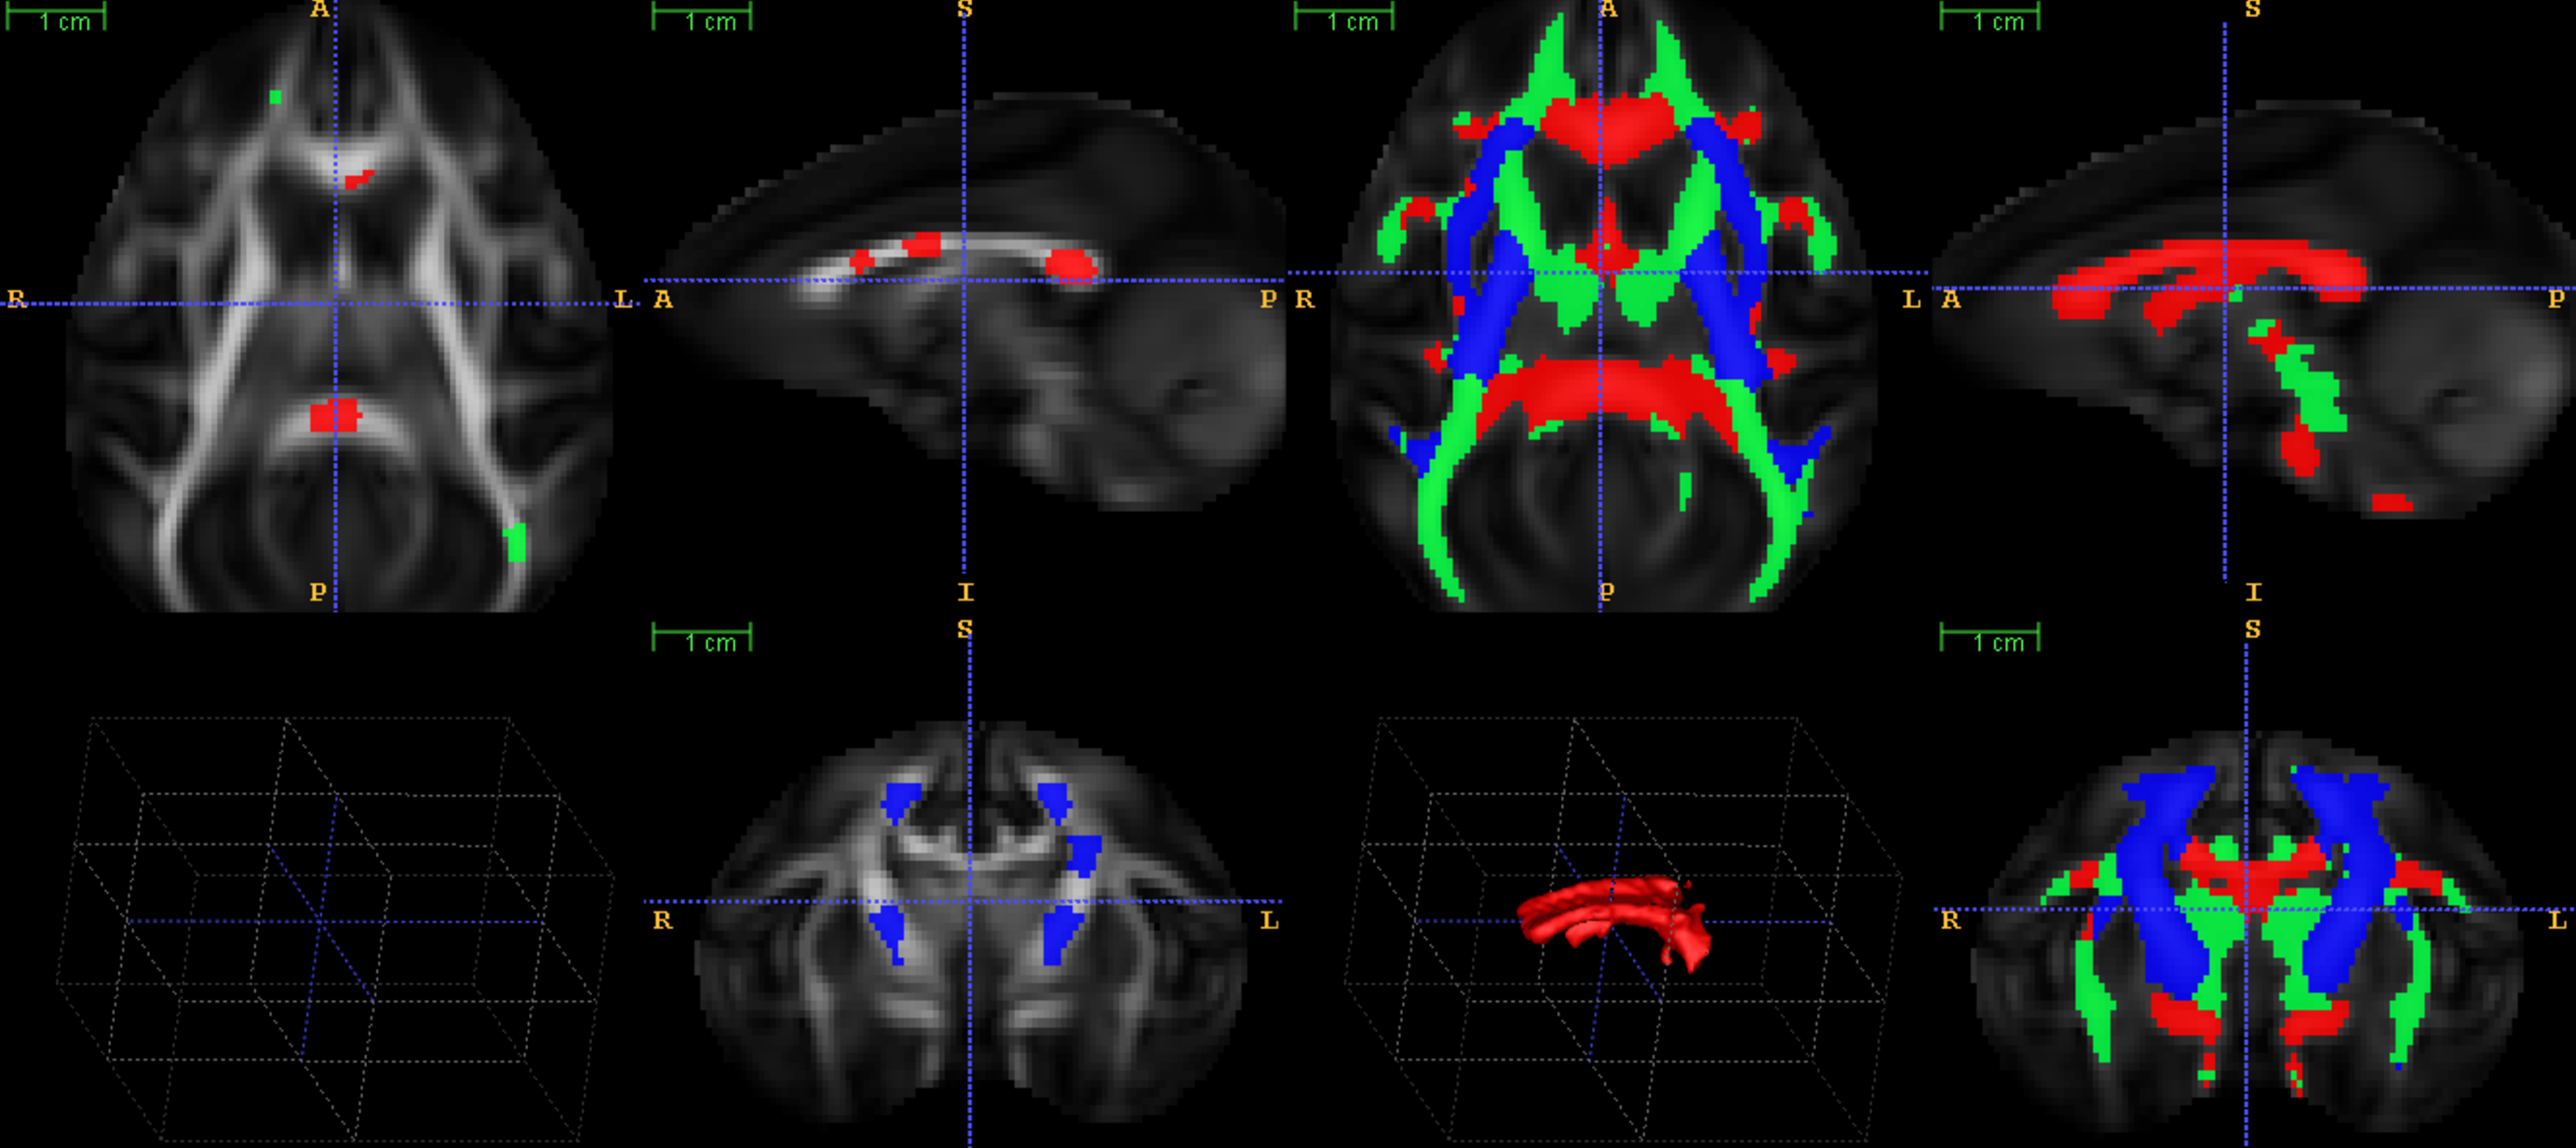
\includegraphics[width=6in]{Figures/macaque_rgb.pdf}
\end{tabular}
\caption{We perform an RGB-based segmentation of the macaque
  population average tensor image.  At left is the manually placed
  labels, as performed in ITK-Snap.  At right is the Atropos result.
  You may repeat this study by labeling the macaque image with labels
  1, 2 and 3 (R, G, B) similarly to this example.  You then
  save the segmentation and run the script entitled MVSeg/src/scripts/seg\_dti\_manual\_init\_atropos.}
\label{fig:macaque}
\end{center}
\end{figure}



\section{Data}
\subsection{DTI}
We can start small with a couple of interesting datasets. 

\noindent $I$ High-resolution human DT atlas in nifti format: \url{http://www.nitrc.org/frs/?group_id=432}

\noindent $J$ A second human DT atlas
\url{http://www.nitrc.org/projects/dtitk} which also has labels that
may be used to guide our parcellation of the white matter into major
tracts.

\noindent $K$ A similar atlas for macaque \url{http://www.nitrc.org/projects/rmdtitemplate}

Segmenting these templates into similar regions will let us quantify
differences in white matter due to aging in humans ($I$ vs $J$) and
between humans and macaques ($I$ and $J$ vs $K$).

Once we establish a working knowledge of DTI segmentation, we can
evaluate reproducibility of our methods on the Kirby dataset
\url{http://www.nitrc.org/projects/multimodal/}.  This unique
collection of images has repeat imaging on the same subject within a
week.  Thus, our segmentation tools should provide repeatable
measurements of volume or tracts across all subjects.  Once
repeatability is established, we can apply the segmentation approach
to other datasets where investigating population differences is of
interest.

\begin{figure}
\begin{center}
\begin{tabular}{c}
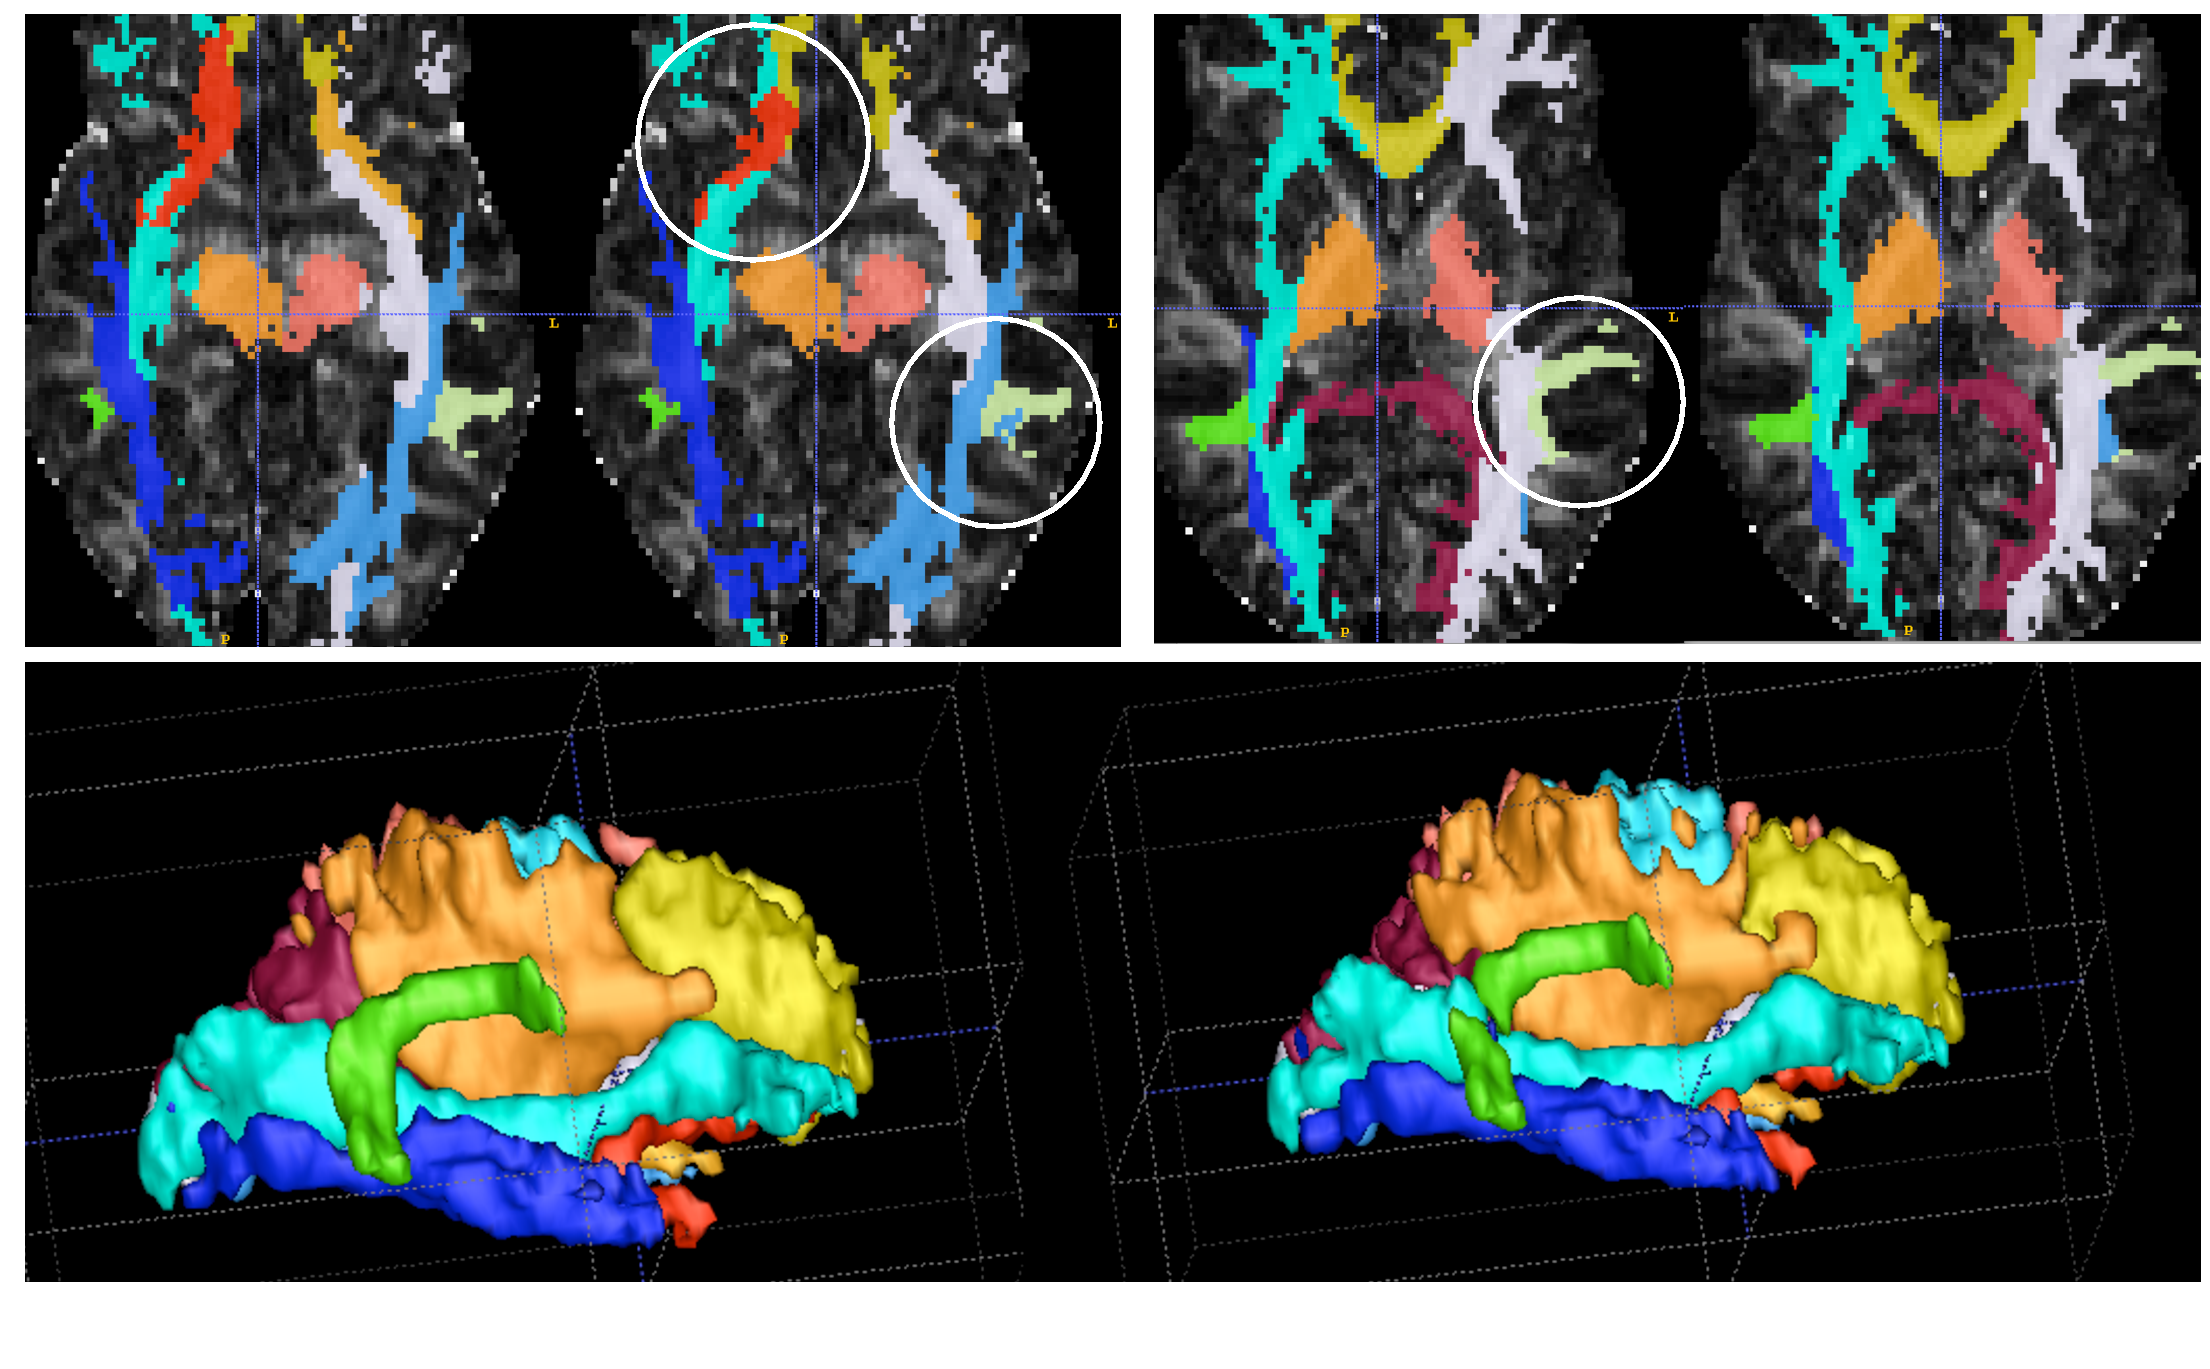
\includegraphics[width=6in]{Figures/004_vec_vs_dti.pdf}
\end{tabular}
\caption{The tensor-based segmentation on the left and the
  RGB vector segmentation is on the right.  Both use Mahalanobis
  distance and EM optimization with spatial priors.}
\label{fig:example1}
\end{center}
\end{figure}

\subsection{Neonate T1 and T2} There is also an interesting neonatal
dataset for which there is some multivariate data (T1 and T2).  The
goal with the neonatal segmentation is to increase repeatability
between automated and manual volume measurements.  We do fairly well
already but could improve results with some additional work on, for
instance, distance metrics and/or partial volume estimation.

\section{Methods} Our goal will be to provide reproducible
measurements derived from multivariate segmentation.  An EM
segmentation method can use any of the DTI features we discussed
above.  One project that may be similar to our own is here
\url{http://www.nitrc.org/projects/dots} though there is no clear
reference other than the website.  Prior DT segmentation work is here
\citep{Lenglet2005} and here \citep{Awate2007}.  Classic work on
partial volume estimation \citep{Santago1993,Shattuck2001}.

\subsection{Ideas}
One idea to explore is nonparametric joint histogram based likelihood
models for tensor shape and orientation.  $J_{orientation} = f(i,j)/
\sum_{ij} f(i,j) $ where $f(i,j)$ is the frequency histogram of the
upper hemisphere describing orientation.  two parameters: theta and
psi.  $J_{shape} = g(i,j)/ \sum_{ij} g(i,j) $ where $g(i,j)$ is the
frequency histogram describing the co-occurrence of first and second
eigenvalues.  These would become our likelihood models (recalling
$P(i|Q)$) and would be initialized by priors deformed from previously
segmented images.

We can also explore the effect of simulated and/or deterministic
annealing which is a hidden feature of Atropos. 

\subsection{Code}
The class called {\em antsHistogramParzenWindowsListSampleFunction}
implements a non-parametric histogram based likelihood function.  It is located in MVSeg/src/ANTS/ImageSegmentation.
One might implement a class called  {\em
  antsJointHistogramParzenWindowsListSampleFunction} that could
implement the idea above.   Or one could follow the example {\em
  antsLogEuclideanGaussianListSampleFunction} to implement a
parametric likelihood.  Each class should be tested as a stand-alone
method and should be verified to work before being included in the
segmentation functionality.  

\section{Results}

\section{Discussion}

\paragraph{Information Sharing Statement}
{Atropos software is available in ANTs
    {\color{blue}{\url{http://www.picsl.upenn.edu/ANTs}}}
which depends on ITK {\color{blue}{\url{http://www.itk.org/Wiki/ITK/Git/Download}}}.
BrainWeb provides good evaluation data
{\color{blue}{\url{http://mouldy.bic.mni.mcgill.ca/BrainWeb/}}}.
ITK-SNAP is useful for scalar and RGB visualization {\color{blue}{\url{www.itksnap.org}}}.

\paragraph{Acknowledgments}
{This work was supported in part by NIH (AG17586, AG15116, NS44266, and
NS53488).}

\newpage

\bibliographystyle{plain}
\bibliography{MVSeg} 
\end{document}
